
%%%%%%%%%%%%%%%%%%%%%%% file typeinst.tex %%%%%%%%%%%%%%%%%%%%%%%%%
%
% This is the LaTeX source for the instructions to authors using
% the LaTeX document class 'llncs.cls' for contributions to
% the Lecture Notes in Computer Sciences series.
% http://www.springer.com/lncs       Springer Heidelberg 2006/05/04
%
% It may be used as a template for your own input - copy it
% to a new file with a new name and use it as the basis
% for your article.
%
% NB: the document class 'llncs' has its own and detailed documentation, see
% ftp://ftp.springer.de/data/pubftp/pub/tex/latex/llncs/latex2e/llncsdoc.pdf
%
%%%%%%%%%%%%%%%%%%%%%%%%%%%%%%%%%%%%%%%%%%%%%%%%%%%%%%%%%%%%%%%%%%%


\documentclass[runningheads,a4paper]{llncs}

\usepackage{amssymb}
\setcounter{tocdepth}{3}
\usepackage{graphicx}
\usepackage{epstopdf}
\usepackage{subfig}

\graphicspath{{images/}}

\usepackage{url}
\urldef{\mailsa}\path|ary506@york.ac.uk|
\newcommand{\keywords}[1]{\par\addvspace\baselineskip
\noindent\keywordname\enspace\ignorespaces#1}

\begin{document}

\mainmatter  % start of an individual contribution

% first the title is needed
\title{Gamification of Software Modelling Learning}

% a short form should be given in case it is too long for the running head
\titlerunning{Gamification of Software Modelling Learning}

% the name(s) of the author(s) follow(s) next
%
% NB: Chinese authors should write their first names(s) in front of
% their surnames. This ensures that the names appear correctly in
% the running heads and the author index.
%
\author{Alfa Yohannis}
%
\authorrunning{Gamification of Software Modelling Learning}
% (feature abused for this document to repeat the title also on left hand pages)

% the affiliations are given next; don't give your e-mail address
% unless you accept that it will be published
\institute{Department of Computer Science, University of York, York, United Kingdom\\
\mailsa\\}

%
% NB: a more complex sample for affiliations and the mapping to the
% corresponding authors can be found in the file "llncs.dem"
% (search for the string "\mainmatter" where a contribution starts).
% "llncs.dem" accompanies the document class "llncs.cls".
%

\toctitle{Lecture Notes in Computer Science}
\tocauthor{Gamification of Software Modelling Learning}
\maketitle


\begin{abstract}
The abstract should summarize the contents of the paper and should
contain at least 70 and at most 150 words. It should be written using the
\emph{abstract} environment.
\keywords{software modelling, gamification, learning}
\end{abstract}


\section{Introduction}
Software modelling is commonly perceived as an difficult subject since it requires a great deal of abstractions \cite{Borstler2012}. However, this subject has a fundamental and crucial role in software engineering. Failure to master this subject will affect the student’s abstraction capability in analysing and designing a real-world software. Less proficiency in software modelling will likely cause software engineering students facing difficulties completing their degrees, as most of the software engineering related subjects have a sense of intrinsic abstraction problems \cite{Kramer2007}. Their perception of software modelling will affect their attitude towards software engineering today and their career paths in the future.

For new software engineering students, software modelling is commonly perceived as subjects that are difficult to learn. Software, by its nature, is abstract and complex that demand loads of abstraction to model it. This problem is similar to problems in mathematics where much of the concepts can only be accessed through symbolical representations \cite{Duval2006}. Abstraction also means requiring the students to perform information hiding, generalization, approximation or reformulation, leaving out the irrelevant aspects but keeping the relevant ones, or separation from the concrete reality \cite{Saitta2013}. In order to overcome these challenges, we need to put more efforts on delivering software modelling in a more concrete and motivating presentation which can engage and ease students to learn it.

On the other hand, the use of games or game elements for serious purposes other than leisure has drawn lots of attentions. Gamification \cite{deterding2011game} and Serious Games \cite{Michael2005} have been viewed as solutions to solve motivational problems that emerge when users engage in  boring, irrelevant, difficult activities, e.g. learning sorting algorithms \cite{Yohannis2015} or C-programming \cite{Ibanez2014}.

Therefore, the purpose of this research is to investigate and develop a gamification design framework that will systematically direct game design to produce a more accurate software modelling gamification yielding better-designed software modelling games. More precisely, this research aims to answer the following research questions that are derived from the general research objective:
\begin{enumerate}
\item Which processes, aspects, and components of software modelling and their teaching and learning practices that are essential to take into account?
\item What types of game elements and their roles that can deliver software modelling at best? 
\item What kind of framework that orchestrates, design the interaction between, software modelling and game elements, to produce a better software modelling gamification?
\item To what extend gamification of software modelling better engage, motivate, and improve learners’ performances?
\end{enumerate}

\section{Related Works}

Several approaches have been conducted to bring software modelling into a more concrete presentation that can be easily understood by learners, ranging from didactic learning (Moisan \& Rigault, 2010), modeling tools utilization (Akayama, et al., 2013), alternative communication channels and the use of modelling language (Brandsteidl, Wieland, \& Huemer, 2011), immersive visual modelling through virtual environment (Neubauer \& Harris, 2003), software design studio (Whittle, Bull, Lee, \& Kotonya, 2014), project-based approach (Szmurło \& Śmiałek, 2007), to code generation investigation (Schmidt, Kimmig, Bittner, \& Dickerhof, 2014). 

However, most of the approaches have weaknesses in motivating learners to engage continuously, frequently, and actively to learn software modelling, which is the important aspect to impact greatly on learning (Naps, 2005). This condition then elevates game as one approach, a.k.a. game-based learning, to learn or teach software modelling. This approach provides students a new way of learning software modelling, which is not only interactive but also engaging enough to keep them learning continuously. 

The use of game elements for a purpose other than leisure is called gamification (Deterding, Dixon, Khaled, \& Nacke, 2011). Regardless gamification design is still an ongoing challenge (Deterding, Björk, Nacke, Dixon, \& Lawley, 2013), it is an opportunity for research that up today there is still no gamification design framework that particularly address how to guide the design of software modelling gamification; a framework that guides how to integrate game specific domain into software modelling. Therefore, this research aims to develop a gamification design framework of software modelling.

Research publications on the application of games or game elements for software modelling are difficult to find. One that exists is the work of Groenewegen et al. that proposed a game dedicated to the learning and teaching of  the validity of a model of software architecture (Groenewegen, Hoppenbrouwers, \& Proper, 2010). However, their work is limited to the validity of software architecture and did not provide a deep comprehension on ‘how’ game elements or mechanics should be integrated into software modelling in general. The gamification of software modelling was not discussed in depth. 

This is in line with the question prompted by (Prensky, 2005) that the ‘how’ of learning games design is essential to be addressed. Likewise, Perotta et al. proposed a research challenge that a more analytic approach need to be developed on how game elements contribute to learning (Perotta, Featherstone, Aston, \& Houghton, 2012), including a better understanding on how games match to desired outcomes and how games integrate into user’s learning experience (Conolly, Boyle, MacArthur, Hainey, \& Boyle, 2012). This condition also aligns to what Deterding et al. also prompted that much work needs to be done on gamification design, how to integrate existing design patterns and dynamics of games into non-game contexts (Deterding, Björk, Nacke, Dixon, \& Lawley, 2013).

These challenges can be interpreted as a focus on design problems that seek how to organize game elements and mechanics to meet certain functionalities or desired results. This focus will open the underlying processes of how games contribute to learning unveiling particular principles on game elements and mechanics. The understanding of the processes and the role of game mechanics will lead to the construction of gamification design frameworks. 

Gamification has been implemented in different fields but the results are predicted will not always as expected and some will end in failures (Gartner, 2012). Therefore, the presence of a gamification design framework for software modelling is imperative since it will direct gameful design to produce a more accurate software modelling gamification yielding better-designed gameful experiences of software modelling. 

Existing gamification frameworks are not adequate as they come from marketing or management backgrounds, not from software engineering discipline, and they provide guidance more to wise-step implementation approach rather than structural and dynamic points of view (Werbach \& Hunter, 2012) (Huang \& Soman, 2013) (Kumar, 2013). The relations between software modelling components and relevant game mechanics and elements are important to be studied, as it will provide a basis for constructing a gamification design framework for software modelling.

\section{Research Methods}
Since the output of this work is design artefacts, we decided to utilise the Design Science Research Methodology (DSRM) \cite{peffers2007design} as our umbrella methodology. DSRM is selected because it provides a comprehensive high-level conceptual framework how to undergo a full-cycle research process. It also provides six-activity guidelines for understanding, developing, executing, and evaluating design artifacts. The six activities are (1) problem identification and motivation activity, (2) define objectives for a solution activity, (3) define objectives for a solution activity, (4) design and development activity, (5) demonstration and evaluation activities, and (6) communication. 

The high-level characteristic means that we can employ other research methods as the sub methods in each activity. For examples, we employ interviews, literature reviews, and discussion with experts as our methods in problem identification and motivation activity as well as utilise Deterding's lens of intrinsic skill atoms \cite{deterding2015lens} to produce a gameful design in the design and development activity. As information, our work is still in the design and development activity and there are three activities remaining to work on. We use the first three activities of DSRM as our guidelines to report our in-progress accomplishment.
 
\section{Problem Identification and Motivation Activity}

\section{Define Objectives and Evaluation Activity}

\section{Design and Development Activity}

\subsection{Game Design}

\begin{figure}[htb]
\centering
\subfloat[Level Selection]{\frame{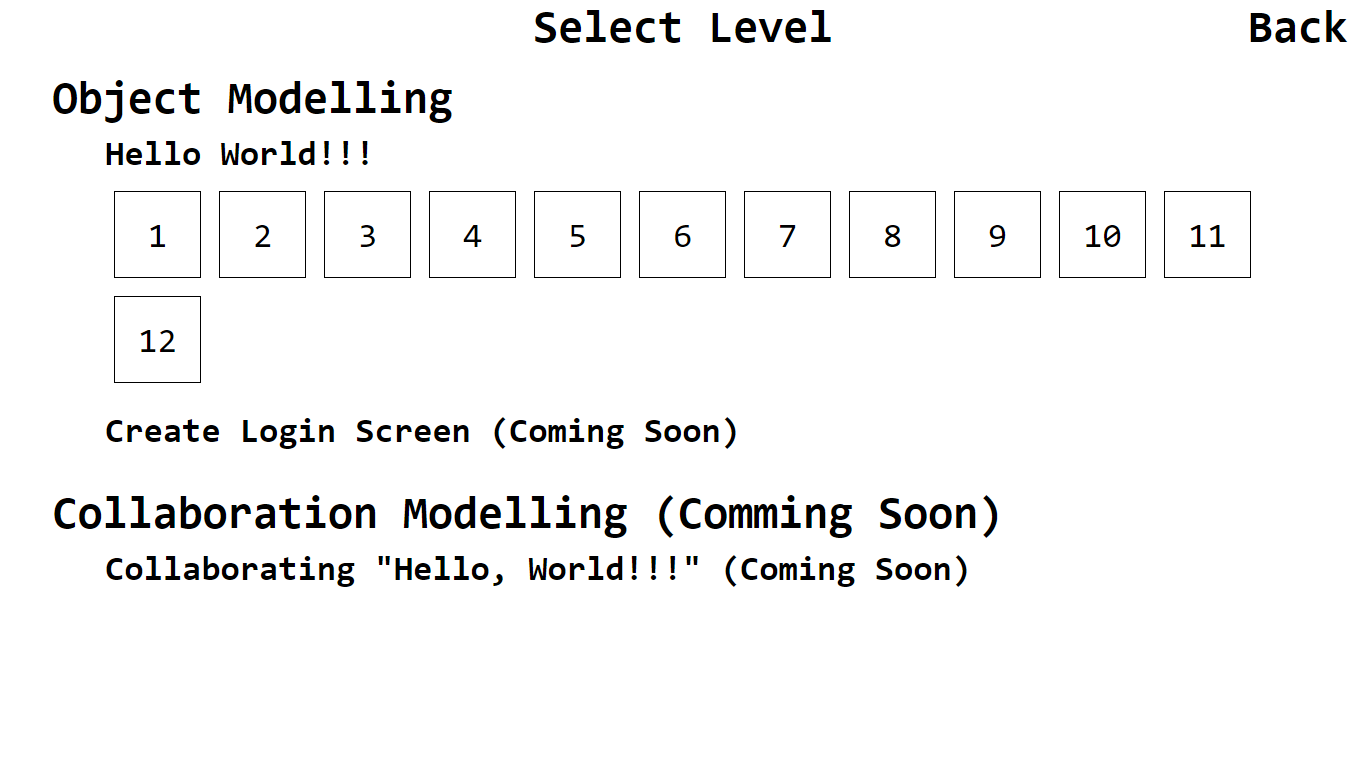
\includegraphics[height=3.5cm]{levels}}}
\hspace*{\fill}
\subfloat[Positive Reinforcement]{\frame{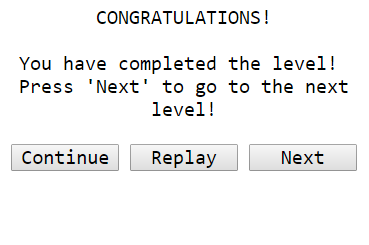
\includegraphics[height=3.5cm]{positive}}}
\caption{Game and learning elements embedded into the artifact.}
\end{figure}

\begin{figure}[htb]
\centering
\frame{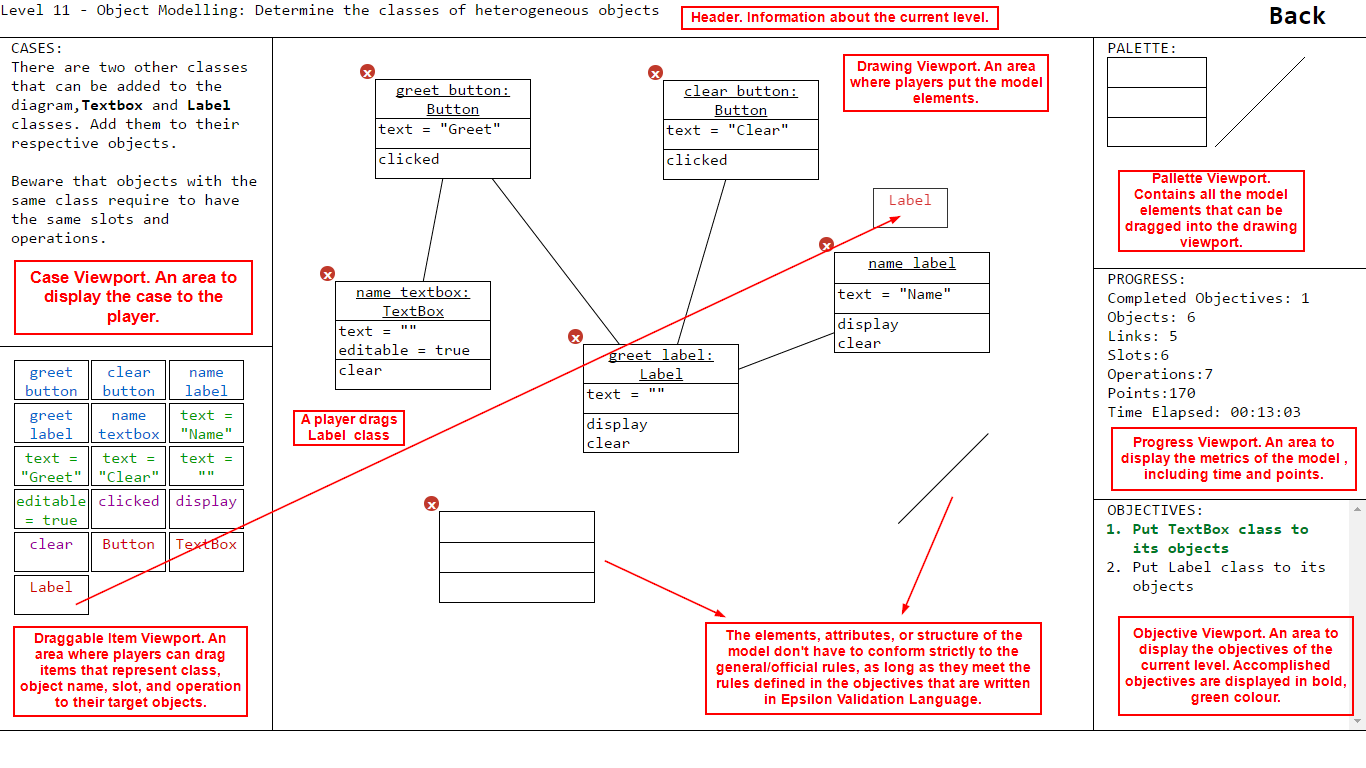
\includegraphics[width=\textwidth]{game-annotated}}
\caption{The game's display.}
\end{figure}

\subsection{Architecture}

\subsection{Modelling Editor}

\begin{figure}[htb]
\centering
\frame{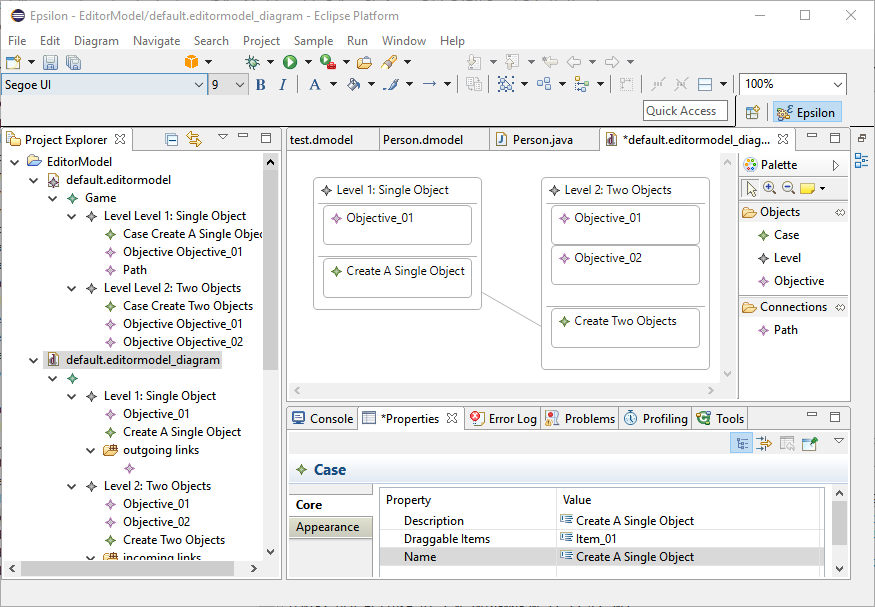
\includegraphics[width=\textwidth]{editor}}
\caption{Game editor to automatically generate the game.}
\end{figure}

\section{Discussion}
In order to develop a gamification design framework of software modelling, the software modelling itself has to be understood at first. By doing so, we can capture the underlying principles that are essential in delivering software modelling and therefore we can develop the framework more accurate. There are many approaches have been conducted so far to learn and to teach software modelling. From those approaches, we can identify important processes, aspects, and components, which without them will bring impairment to the software modelling, and use them as the consideration in developing the framework. 

Successfully identifying the underlying principles, processes, aspects, and components of software modelling is worthless without mapping them to representative game elements. Consequently, identifying representative types of game elements is a crucial effort to represent the software modelling within the gamification. As a result, more options are available in balancing the presence of the ‘seriousness’ of software modelling and the ‘fun’ delivered by the game elements in the gamification design.

Mapping software modelling and game elements is not a trivial task. The interaction between them needs to be identified. It is a kind of relationship that both software modelling and game elements can present at the same time while the user is interacting with a representative design artefact. Understanding the relationship will enable us to develop a framework that can orchestrate, design the interaction between, software modelling and game elements to produce a better software modelling gamification.

A working artifact, as the embodiment of the framework, has to be constructed, applied, and then evaluated in several case studies. It is the way we validate the framework since the artifact is the indirect representation of the framework. Measuring the artifact’s outcomes will also measure the impact of the framework. The results of the validation will be the inputs to improve the artifact and mainly to revise and refine the gamification design framework of software modelling.

\section{Conclusion}
 

\subsubsection*{Acknowledgments.} We would like to thank our respondents that participated in our preliminary interview. This research is supported by \emph{Lembaga Pengelola Dana Pendidikan Indonesia} (Indonesia Endowment Fund for Education). 

Test Citing \cite{deterding2011game}

\bibliography{references} 
\bibliographystyle{ieeetr}




\section*{Appendix A: Interview Questions}


\end{document}

